\documentclass[12pt]{report}
\usepackage[a4paper,top=15mm, bottom=25mm, left=23mm, right=23mm]{geometry}
\usepackage[english]{babel}
\usepackage[utf8]{inputenc}
\usepackage{mathptmx}
\usepackage{amssymb}
\usepackage{amsmath}
\usepackage{enumitem}
\usepackage{tikz}
\usepackage{stuki}

\renewcommand{\labelitemi}{$-$}
\renewcommand{\labelitemii}{}

\usetikzlibrary{arrows,shapes,positioning,shadows,trees}

\tikzset{
  basic/.style  = {draw, text width=3cm, drop shadow, font=\sffamily, rectangle},
  root/.style   = {basic, rounded corners=2pt, thin, align=center,
                   fill=blue!30},
  level 2/.style = {basic, rounded corners=6pt, thin,align=center, fill=blue!20,
                   text width=15em}
}

\begin{document}
\begin{tabular}{lcr}
\textbf{Lestár Norbert} & 0. beadandó / 11. feladat  & 2015. március 03. \\
\textbf{Neptun kód:} A8UZ7T \\
lestar.norbert@gmail.com \\
6. csoport \\
\end{tabular}
\paragraph{Feladat} \hspace{0pt} \\
\textit{Keressük meg a legmagasabb völgyet a mérési sorozatban!}
\paragraph{Specifikáció} \hspace{0pt} \\
A méréseket egy tömbben tároljuk. \newline
A = ( t : Int$^{n}$, maxh : $\mathbb{N}$, l:$\mathbb{L}$ ) \newline
Ef = ( t = t' ) \newline
Uf = ( Ef $\wedge$ l = $\exists$ (i $\in$ [1..n] $\wedge$ maxh = f(i) $\wedge \forall$ j $\in$ [1..n] : $\beta$(j) $\Rightarrow$ f(j) $\leq$ f(i)) ) = \\ ( Ef $\wedge$ (maxh, l) = $\max\limits_{\substack{i=2 \\ \beta(i)}}^{n-1}$ f(i) ) \newline
ahol $\beta$(i) := f(i-1) $>$ f(i) $<$ f(i+1)
\paragraph{Algoritmus} \hspace{0pt} \\
A feladatot a feltételes maximum keresés programozási tételére vezetjük vissza. Mivel a tételben szereplő index nem fontos a feladat szempontjából, ezért az ind:=i értékadás elhagyható az algoritmusból. \newline
\begin{tabular}{c}
m..n $\rightarrow$ 2..n-1 \\
max $\rightarrow$ maxh \\
f(i) $\rightarrow$ t$_{i}$ \\
$\beta$(i) $\rightarrow$ t$_{i-1}$ $>$ t$_{i}$ $<$ t$_{i+1}$
\end{tabular}

\begin{stuki}[14cm]
\stm*{l := hamis}
\begin{WHILE}{3}{\stm*{i = 2 .. n-1}}
\begin{CASE}{2}{6}
\WHEN[2]{
\stm[1]{ \neg \beta (i) }
}
\stm{SKIP}
\WHEN[2]{
\stm[1]{ \beta (i) \wedge l}
}
\begin{IF}{1}{\stm*{maxh $<$ t[i]}}
\stm*{maxh := t[i]}
\ELSE
\stm*{SKIP}
\end{IF}
\WHEN[2]{
\stm[1]{ \beta (i) \wedge \neg l }
}
\stm{ l := igaz }
\stm{ maxh := t[i]}
\end{CASE}
\end{WHILE}
\end{stuki}

\paragraph{Implementáció} \hspace{0pt} \\

\textit{\textbf{Adattípusok megvalósítása}} \newline
A kódoláskor a t tömböt vector$<$int$>$-ként deklaráljuk, amelynek mérete t.size() alakban érhető el. Mivel a vektor 0-tól indexelődik, ezért a tervbeli ciklus nem a 2..n-1, hanem a 1..t.size()-1 intervallumot futja be, aminek következtében a struktogramm kódja az alábbi lesz:\\
    bool l = false; \\
    int maxh; \\
    for(vector$\_$size i=1; i$<$t.size()-1; ++i)$\lbrace$ \\
         if (!(t[i-1] $>$ t[i] $\& \&$ t[i+1] $>$ t[i])) continue; \\
         if (l) $\lbrace$ \\
             if (maxh $<$ t[i]) maxh = t[i]; \\
         $\rbrace$ else $\lbrace$ \\
             l = true; maxh = t[i]; $\rbrace$ $\rbrace$ \\

\textit{\textbf{Bemenő adatok formája}} \newline
A bemenő adatokat egy szöveges állományból kell a tömbbe bemásolni. Az állományban a megadott számokat szóközökkel, tabulátor jelekkel vagy sorvége jelekkel elválasztva kell beírni. Az állomány minden sorát sorvége jel zárja le. Alapesetben a program csak természetes számokat vár, ám szöveget tartalmazó sorokat/egységeket is lekezeli. Például:\\
1500	150 \newline
250 \newline
-500

\textit{\textbf{Függvények kapcsolódási szerkezete}} \newline
A kódban több függvényt is használunk. A searchmax() tartalmazza a tervben leírt feltételes maximumkeresést, a readfile() tölti fel egy szöveges állományból a tömböt számokkal és írja ki azokat a könnyebb hibakeresés végett, valamint ezeket a függvényeket a main() hívja meg, amely az eredmény kiírását is végzi. \newline
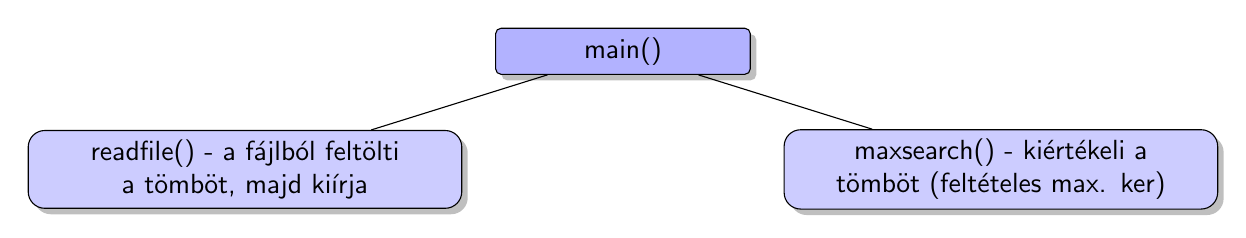
\begin{tikzpicture}[
  level 1/.style={sibling distance=96mm},
  edge from parent/.style={-,draw},
  >=latex]

% root of the the initial tree, level 1
\node[root] {main()}
% The first level, as children of the initial tree
  child {node[level 2] (c1) {readfile() - a fájlból feltölti a tömböt, majd kiírja}}
  child {node[level 2] (c7) {maxsearch() - kiértékeli a tömböt (feltételes max. ker)}};


\end{tikzpicture}
\paragraph{Tesztelési terv} \hspace{0pt} \\

\textit{\textbf{A feladat specifikációjára épülő (fekete doboz) tesztesetek:}}
\begin{itemize}[noitemsep]
\item \textbf{Feltételes maximum keresés} tesztesetei:
\begin{itemize}[noitemsep]
\item \textbf{intervallum hossza} szerint
\begin{enumerate}[noitemsep]
\item \textit{nulla} hosszú: Egyetlen szám sincs. (üres vagy csak elválasztójelekből álló fájl - t3.txt: [] – Nincsen feltöltve a tömb, így maximum sincs.) 
\item \textit{egy} hosszú: Egyetlen szám van. (t10.txt - Legalább három elem kell a feltétel teljesüléséhez, így nem lesz maximum.)
\item \textit{három} hosszú: Három szám van. (t8.txt [2000, 500, 2000] - a maximum az 500 lesz.)
\item \textit{több} hosszú: Több szám van. (t9.txt [2100, 300, 2100, 650, 2200] - a maximum 650 lesz.)
\end{enumerate}
\end{itemize}
\begin{itemize}[noitemsep]
\item \textbf{intervallum eleje} szerint
\begin{enumerate}[noitemsep]
\item A maximum a legelső vizsgált elem. (t8.txt [2000, 500, 2000] - a maximum 500 lesz.)
\end{enumerate}
\end{itemize}
\begin{itemize}[noitemsep]
\item \textbf{intervallum vége} szerint
\begin{enumerate}[noitemsep]
\item A maximum a legutolsó vizsgált elem. (t9.txt [2100, 300, 2100, 650, 2200] - a maximum 650 lesz.)
\end{enumerate}
\end{itemize}
\begin{itemize}[noitemsep]
\item \textbf{tételre jellemző} esetek
\begin{enumerate}[noitemsep]
\item Egyetlen feltételnek eleget tevő szám van. (t8.txt [2000, 500, 2000] - a maximum 500 lesz.)
\item Kettő feltételnek eleget tevő szám van. (t9.txt [2100, 300, 2100, 650, 2200] - a maximum 650 lesz.)
\item Több, a feltételnek eleget tevő szám van. (t2.txt [1000, 200, 1300, 750, 1500, 4500, 500, 5000, 7000] - a maximum 750 lesz.)
\end{enumerate}
\end{itemize}
\item \textbf{Különleges értékek} esetei:
\begin{enumerate}[noitemsep]
\item Üres sorok, nem természetes számokból vagy szövegekből álló adatok. (Ezt a beolvasás figyelmen kívül hagyja)
\end{enumerate}
\end{itemize}

\textit{\textbf{A megoldó programra épülő (fehér doboz) tesztesetek:}}
\begin{enumerate}[noitemsep]
  \item Hibás vagy nem létező állománynév megadása.
  \item Ismételt futtatás kipróbálása.
  \item Olyan állomány olvasása, ahol egy sorban több szám is található egyetlen illetve több szóközzel vagy tabulátor jellel elválasztva. (t6.txt)
  \item Olyan állomány olvasása, ahol minden szám külön sorban van. (t1.txt)
  \item Főprogram ciklusának ellenőrzése: olyan bemenő adatokkal, amelyekre a ciklus egyszer sem fut le (t3.txt), pontosan egyszer fut le (t7.txt), többször lefut és pozitív értéket ad (t2.txt).
\end{enumerate}
\end{document}